\documentclass[12pt, twoside]{article}
\usepackage{titlesec, fancyhdr, float, mathtools, amsmath, amssymb, amsthm, enumitem, mleftright, tikz, pgfplots, scrextend, lipsum}
\usepackage[makeroom]{cancel}
\usepackage[margin = 1in]{geometry}
\usepackage[allcolors = black, colorlinks]{hyperref}

%%%%%%%%%%%%%%%%%%%%%%%% Definitions and formatting
\newcommand{\p}[1]{\mleft( #1 \mright)}
\newcommand{\abs}[1]{\mleft| #1 \mright|}
\newcommand{\diff}[1]{\mathrm{d}#1}
\newcommand{\noskip}
{
	\setlength\abovedisplayskip{0pt}
	\setlength\belowdisplayskip{0pt}
}
\newcommand{\normalskip}
{
	\setlength\abovedisplayskip{\baselineskip}
	\setlength\belowdisplayskip{\baselineskip}
}
\renewcommand{\contentsname}{Table of Contents}
\titlespacing*{\subsection}{0pt}{\baselineskip}{0.5\baselineskip}
\titlespacing*{\section}{0pt}{\baselineskip}{0.5\baselineskip}
\setlength\parindent{0pt}
\raggedbottom

%%%%%%%%%%%%%%%%%%%%%%%% Plot formatting
\def\slopecolor{blue!80!white}

%%%%%%%%%%%%%%%%%%%%%%%% Custom environments
\newenvironment{example}
{
	\textit{Example:}
	\begin{addmargin*}{0.25in}
}
{
	\end{addmargin*}
}

%%%%%%%%%%%%%%%%%%%%%%%% Theorem environments
\makeatletter
\def\thm@space@setup%
{%
	\thm@preskip = \baselineskip
	\thm@postskip = \baselineskip
}
\newtheorem{theorem}{Theorem}[section]
\newtheorem{corollary}{Corollary}[theorem]
\theoremstyle{definition}
\newtheorem*{definition}{Definition}
\newtheorem*{remark}{Remark}

\begin{document}

\noskip

%%%%%%%%%%%%%%%%%%%%%%%% Title page and table of contents
\pagestyle{empty}
\begin{center}
	\vspace*{10\baselineskip}
	\LARGE MATH 33B \\
	\Large Steven Truong
\end{center}
\cleardoublepage

\tableofcontents
\cleardoublepage
\setcounter{page}{1}

%%%%%%%%%%%%%%%%%%%%%%%% Readjusting the layout of the page
\newgeometry{outer = 1in, inner = 0.5in}
\pagestyle{fancy}
\fancyhf{}
\renewcommand{\sectionmark}[1]{\markright{#1}}
\fancyhead[LE, RO]{\thepage}
\fancyhead[RE, LO]{\rightmark}

%%%%%%%%%%%%%%%%%%%%%%%% Beginning of study guide
\section{Introduction}%
\subsection{Ordinary Differential Equations}
\begin{definition}
	An ordinary differential equation is an equation involving a function of a single variable and its derivatives.
\end{definition}
\begin{example}
	\vspace{-\baselineskip}
	\begin{flalign*}
		& y' = y & \\
		& y' = y^2 - t \\
		& y'' + y' = ye^t
	\end{flalign*}
\end{example}
\subsection{Normal Forms}
\begin{definition}
	A first order equation $y' = f\p{t, y}$ is said to be in normal form. More generally, $y^{(n)} = f\p{t, y^{(1)}, y^{(2)}, \ldots, y^{(n-1)}}$ is in normal form.
\end{definition}
\begin{example}
The normal form of $y' + 2ty = 0$ is given by $y' = -2ty$.
\end{example}
\par\bigskip
Differential equations can have many solutions. In the above equation, all solutions are in the form $y\p{t} = Ce^{-t^2}$, so it is called the \textit{general solution} to the above ODE.
\begin{definition}
	The general solution is the family of solutions depending on some parameters that give all but a finite number of solutions.
\end{definition}

\subsection{Initial Value Problems}
\begin{definition}
	A first order ODE $y' = f\p{t, y}$ together with the initial value $y\p{t_0} = y_0$ is called an initial value problem (\textrm{abbreviated as IVP}).
\end{definition}
A solution to an initial value problem satisfies both the associated ODE and the initial condition.

From the above example, if we had the initial condition $y\p{0} = 2$, then the solution to the initial value problem would be $y\p{t} = 2e^{-t^2}$.

\pagebreak
\subsection{Interval of Existence}
\begin{definition}
	Suppose $y = y\p{t}$ satisfies an initial value problem with initial condition $y\p{t_0} = y_0$. Then the interval of existence is the largest interval containing $t = t_0$ on which $y\p{t}$ is defined.
\end{definition}
\begin{example}
	\vspace{-0.5\baselineskip}
	\begin{flalign*}
		&
		\begin{cases}
			y' = y^2 \\
			y\p{0} = 2
		\end{cases}
		&
	\end{flalign*}
	Solution: $\displaystyle y\p{t} = \frac{1}{\frac{1}{2} - t}$
	
	The interval of existence for this IVP is $\p{-\infty, \, \frac{1}{2}}$ (as opposed to the set $\mathbb{R} - \left\{ \frac{1}{2} \right\}$, which is not connected).
\end{example}

\subsection{Geometric Meaning}
Consider $y' = f\p{t, y}$ with $y\p{t_0} = y_0$. If $y\p{t}$ is a solution to the problem, then for any $t$, we must have $\underbrace{y'\p{t}}_{\mathclap{\substack{\text{Slope of } \\ \text{tangent line at }t.}}} = f\p{t, y\p{t}}$.

\subsection{Direction Fields}
\begin{definition}
	A direction field is a plot of line segments, where each one is centered at a point $\p{t, y}$ whose slope is given by $f\p{t, y}$.
\end{definition}
\textit{Example:} $y' = y$
\par
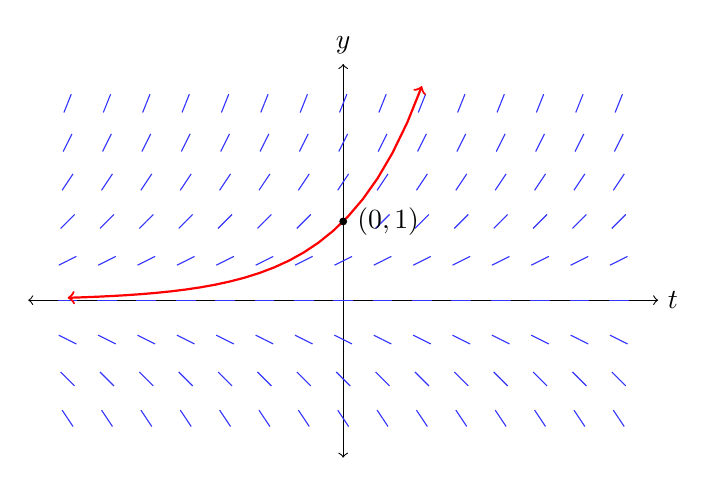
\begin{tikzpicture}
	\draw[<->, black] (-4, 0) -- (4, 0) node[pos = 1, right]{$t$};
	\draw[<->, black] (0, -2) -- (0, 3) node[pos = 1, above]{$y$};
	\foreach \x in {-3.5, -3, ..., 3.5}
		\foreach \y in {-1.5, -1, ..., 2.5}
		{
			\draw[\slopecolor] (\x, \y) -- +({atan(\y)}:-0.125);
			\draw[\slopecolor] (\x, \y) -- +({atan(\y)}:0.125);
		}
	\draw[<->, red, thick, domain = -3.5:1] plot (\x, {exp(\x)});
	\node[circle, inner sep = 1pt, fill = black, label = right:{$\p{0, 1}$}] at (0, 1) {};
\end{tikzpicture}
\par
These are useful for finding numerical solutions to equations we can't solve explicitly.

\subsection{Qualitative Methods}
\textit{Example:} $y' = 1 - y^2$
\par
\begin{figure}[H]
	\begin{minipage}[t]{0.5\textwidth}
		\centering
		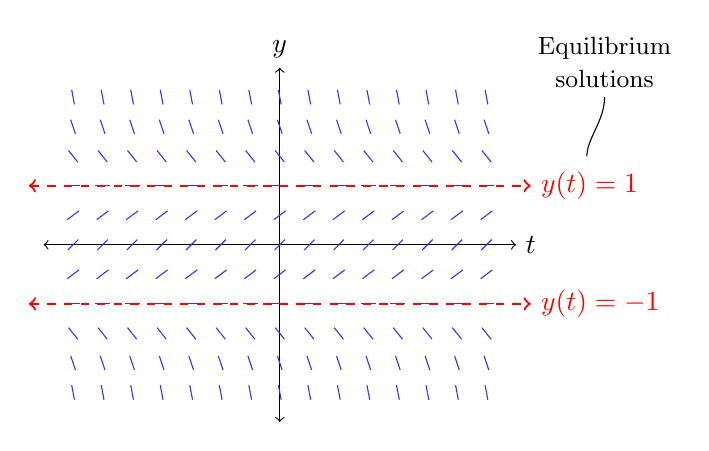
\begin{tikzpicture}[scale = 0.75]
			\draw[<->, black] (-4, 0) -- (4, 0) node[pos = 1, right] {$t$};
			\draw[<->, black] (0, -3) -- (0, 3) node[pos = 1, above] {$y$};
			\foreach \x in {-3.5, -3, ..., 3.5}
				\foreach \y in {-2.5, -2, ..., 2.5}
				{
					\draw[\slopecolor] (\x, \y) -- +({atan(1 - \y * \y)}:-0.125);
					\draw[\slopecolor] (\x, \y) -- +({atan(1 - \y * \y)}:0.125);
				}
			\draw[<->, dashed, thick, red] (-4.25, 1) -- (4.25, 1) node[pos = 1, right] {$y\p{t} = 1$};
			\draw[<->, dashed, thick, red] (-4.25, -1) -- (4.25, -1) node[pos = 1, right] {$y\p{t} = -1$};
			\draw[thin] (5.2, 1.5) .. controls (5.2, 1.8) and (5.5, 2.1) .. (5.5, 2.5) node[pos = 1, above, align = center] {\small Equilibrium \\ \small solutions};
		\end{tikzpicture}
		\caption{Direction Field}
	\end{minipage}%
	\begin{minipage}[t]{0.5\textwidth}
		\centering
		\begin{tikzpicture}[scale = 1.5]
			\draw[<->, black] (-2, 0) -- (2, 0) node[pos = 1, right] {$y$};
			\draw[<->, black] (0, -1.5) -- (0, 1.5) node[pos = 1, above] {$y'$};
			\draw[thin, gray] (-1, -0.25) -- (-1, 0.25) node[pos = 0, below, black] {-1};
			\draw[thin, gray] (1, -0.25) -- (1, 0.25) node[pos = 0, below, black] {1};
			\draw[<->, red, thick] plot[domain = -1.5:1.5] (\x, 1 - \x * \x);
		\end{tikzpicture}
		\caption{Phase Portrait}
	\end{minipage}
\end{figure}
\begin{minipage}[t]{0.5\textwidth}
	Solution classifications:
	\begin{enumerate}[label = \arabic*.]
		\item Equilibrium solution: $y\p{t} = 1$, $y\p{t} = -1$
		\item $\phantom{|} y\p{0} \phantom{|} > 1$: \quad
			\begin{tikzpicture}[scale = 0.35, baseline = -0.8ex]
				\draw[red] (1.25, -0.75) .. controls (-1.3, -0.65) .. (-1.5, 0.5);
			\end{tikzpicture}
		\item $|y\p{0}| < 1$: \quad
			\begin{tikzpicture}[scale = 0.35, baseline = -0.8ex]
				\draw[red] (1.25, 0.5) .. controls (-0.25, 0.5) and (-0.25, -0.75) .. (-1.5, -0.75);
			\end{tikzpicture}
		\item $\phantom{|} y\p{0} \phantom{|} < 1$: \quad
			\begin{tikzpicture}[scale = 0.35, baseline = -0.8ex]
				\draw[red] (1.25, -0.75) .. controls (0.9, 0.5) .. (-1.5, 0.5);
			\end{tikzpicture}
	\end{enumerate}
\end{minipage}%
\begin{minipage}[t]{0.5\textwidth}
	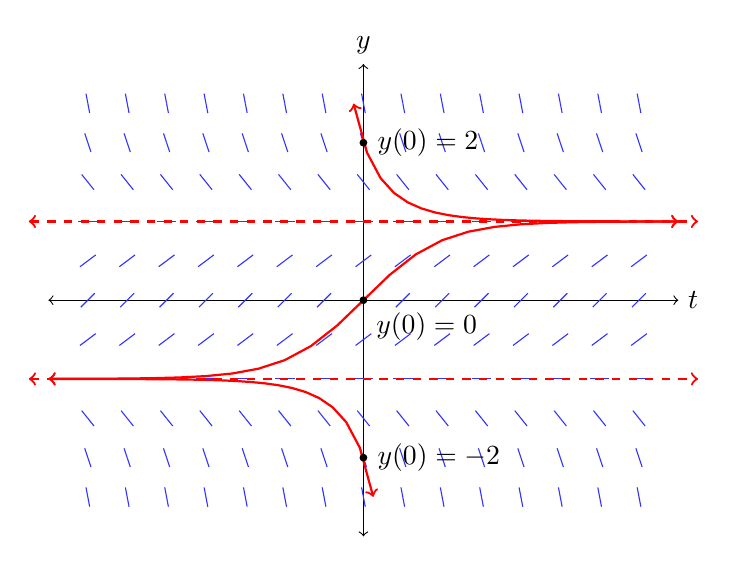
\begin{tikzpicture}[baseline = (current bounding box.north)]
		\draw[<->, black] (-4, 0) -- (4, 0) node[pos = 1, right] {$t$};
		\draw[<->, black] (0, -3) -- (0, 3) node[pos = 1, above] {$y$};
		\foreach \x in {-3.5, -3, ..., 3.5}
			\foreach \y in {-2.5, -2, ..., 2.5}
			{
				\draw[\slopecolor] (\x, \y) -- +({atan(1 - \y * \y)}:-0.125);
				\draw[\slopecolor] (\x, \y) -- +({atan(1 - \y * \y)}:0.125);
			}
		\draw[<->, dashed, thick, red] (-4.25, 1) -- (4.25, 1) node[pos = 1, right] {};
		\draw[<->, dashed, thick, red] (-4.25, -1) -- (4.25, -1) node[pos = 1, right] {};
		\draw[<->, thick, red] plot[domain = -0.125:4] (\x, {(3 * exp(2 * \x) + 1) / (3 * exp(2 * \x) - 1)});
		\node[circle, inner sep = 1pt, fill = black, label = right:{$y\p{0} = 2$}] at (0, 2) {};
		\draw[<->, thick, red] plot[domain = -4:4] (\x, {(exp(2 * \x) - 1) / (exp(2 * \x) + 1)});
		\node[circle, inner sep = 1pt, fill = black, label = below right:{$y\p{0} = 0$}] at (0, 0) {};
		\draw[<->, thick, red] plot[domain = -4:0.125] (\x, {(exp(2 * \x) + 3) / (exp(2 * \x) - 3)});
		\node[circle, inner sep = 1pt, fill = black, label = right:{$y\p{0} = -2$}] at (0, -2) {};
	\end{tikzpicture}
\end{minipage}

\clearpage
\section{Separable Equations}
\subsection{Motivation}
\begin{definition}
	A first order ordinary differential equation is called \textit{separable} if it can be written in the form $y' = f\p{t}g\p{y}$.
\end{definition}
Separable equations appear relatively often in real life. One scenario is in radioactive decay of nuclei.
\par\bigskip
Suppose $N\p{t}$ is the amount of a nuclei at a time $t$. In our model, we assume that the amount of decay is proportional to the amount of nuclei $N$ and the length of time $\Delta t$. Then
\normalskip
\begin{align*}
	\Delta N &= N\p{t + \Delta t} - N\p{t} \approx -\lambda N\p{t} \Delta t \\
		  N' &= \lim_{\Delta t\to0} \frac{N\p{t + \Delta t} - N\p{t}}{\Delta t} = -\lambda N
\end{align*}
The equation can then be solved as follows:
\begin{align*}
	N' &= -\lambda N \\
	\frac{\diff{N}}{\diff{t}} &= -\lambda N \\
	\frac{\diff{N}}{N} &= -\lambda \, \diff{t}, \qquad N \neq 0\text{, but note that it is a solution to the ODE} \\
	\int \frac{\diff{N}}{N} &= \int -\lambda \, \diff{t} \\
	\ln\abs{N} &= -\lambda t + C_0 \\
	\abs{N} &= Ce^{-\lambda t}, \qquad C = e^{C_0} > 0 \\
	N &=
	\begin{cases}
		\phantom{-}Ce^{-\lambda t}, & N\p{t_0} > 0 \\
		-Ce^{-\lambda t}, & N\p{t_0} < 0
	\end{cases}
\end{align*}
If we allow $C$ to take on any real value, then the general solution to the ODE can be written as \[ N\p{t} = Ce^{-\lambda t}. \]
\clearpage
\begin{example}
	\noskip
	\begin{flalign*}
		y' &= t^2y^2 \\
		\frac{\diff{y}}{y^2} &= t^2 \, \diff{t} \\
		\int \frac{\diff{y}}{y^2} &= \int t^2 \, \diff{t} \\
		-\frac{1}{y} &= \frac{1}{3}t^3 + C \\
		y &= -\frac{1}{\frac{1}{3}t^3 + C}
	\end{flalign*}
	Note that $y\p{t} = 0$ is also a solution.
\end{example}

\subsection{``Proof''}
Suppose we have the separable ODE \[ y' = \frac{f\p{t}}{g\p{y}}. \] Then
\normalskip
\begin{align*}
	g\p{y} y' &= f\p{t} \\
	\int g\p{y} y' \, \diff{t} &= \int f\p{t} \, \diff{t} \\
	\int g\p{y} \, \diff{y} &= \int f\p{t} \, \diff{t}, \qquad y = y\p{t} \implies \diff{y} = \frac{\diff{y}}{\diff{t}} \, \diff{t}
\end{align*}
which is the same result from using separation of variables.

\subsection{Using Definite Integration (Newton's Law of Cooling)}
Newton's Law of Cooling states that the change in temperature of an object over time is directly proportional to the difference between the object's current temperature $T$ and the ambient temperature $A$. Mathematically, \[ \frac{\diff{T}}{\diff{t}} = -k\p{T - A}. \] Suppose we had the initial condition $T\p{t_0} = T_0$. Then we can solve the IVP using separation of variables:
\begin{align*}
	\frac{\diff{T}}{\diff{t}} &= -k\p{T - A} \\
	\frac{\diff{T}}{T - A} &= -k \, \diff{t}
\end{align*}
Instead of finding the general solution and then solving for the constant, we can use definite integration to get the particular solution directly. As time goes from $t_0$ to $t$, temperature goes from $T_0$ to $T\p{t}$. Thus,
\begin{align*}
	\int_{T_0}^{T\p{t} }\frac{\diff{u}}{u - A} &= \int_{t_0}^{t} -k \, \diff{v} \\
	\ln\abs{T - A} - \ln\abs{T_0 - A} &= -k\p{t - t_0} \\
	T\p{t} &= A + \p{T_0 - A}e^{-k\p{t - t_0}}
\end{align*}

\subsection{Implicitly Defined Solutions}
Sometimes, we are unable to find an explicit solution to an ODE. I.e., we are unable to get a solution in the form of $y\p{t} = f\p{t}$. Consider the separable differential equation \[ y' = \frac{g\p{t}}{f\p{y}} \] and that $f\p{y}$ and $g\p{t}$ have antiderivatives $F\p{y}$ and $G\p{t}$, respectively. Separation of variables yields
\begin{align*}
	\int f\p{y} \, \diff{y} &= \int g\p{t} \, \diff{t} + C \\
	F\p{y} &= G\p{t} + C \\
	y &= F^{-1}\p{G\p{t} + C}
\end{align*}
If we are unable to find $F^{-1}$, then we will not be able to find an explicit solution for the differential equation.
\par\pagebreak
\begin{example}
	\noskip
	\begin{align*}
		x' &= \frac{x^2}{\p{1 + x}t} \\
		\int \frac{1}{x^2} + \frac{1}{x} \, \diff{x} &= \int \frac{1}{t} \, \diff{t} \\
		-\frac{1}{x} + \ln\abs{x} &= \ln\abs{t} + C
	\end{align*}
	We are unable to solve for $x$, so we cannot find an explicitly defined solution.
\end{example}

\section{Linear Equations}
\subsection{Introduction}
\begin{definition}
	A first order linear differential equation is given by $x' = a\p{t}x + f\p{t}$. If $f\p{t} = 0$, then the equation is said to be \textit{homogeneous}. Otherwise, it is said to be \textit{inhomogeneous}.
\end{definition}
\begin{minipage}[t]{0.5\textwidth}
	\textit{Examples:}
	\vspace{-\baselineskip}
	\begin{addmargin}{0.25in}
		\noskip
		\begin{flalign*}
			& x' = tx + t^2 & \\
			& x' = \p{\frac{\sin{t}}{t} + e^t}x + e^{t^2}
		\end{flalign*}
	\end{addmargin}
\end{minipage}%
\begin{minipage}[t]{0.5\textwidth}
	\textit{Non-examples:}
	\vspace{-\baselineskip}
	\begin{addmargin}{0.25in}
		\noskip
		\begin{flalign*}
		 	& x' = x^2 & \\
			& xx' = \sin{t} \\
			& x' = \sin{x}
		\end{flalign*}
	\end{addmargin}
\end{minipage}%

\subsection{Solutions to Homogeneous Linear Equations}
\normalskip
Homogeneous first order linear differential equations are of the form $x' = a\p{t}x$. Notice that it is separable, and that the general solution is given by \[ x\p{t} = Ce^{\int a\p{t} \, \diff{t}}, \text{ where } C \in \mathbb{R}. \]

\subsection{Solutions to Inhomogeneous Equations}
\subsubsection{Integrating Factors}
Consider the simple inhomogeneous equation \[ x' + x = A. \] The appearance of the $+$ sign and a derivative reminds us of the product rule. As the equation stands, we can't write it as a derivative of a product. However, if we multiply it by some function, we will be able to. The integrating factor for this particular differential equation is $e^x$. Notice that $\p{e^x x}' = e^x x' + e^x x$. Then
\begin{align*}
	e^x x' + e^x x &= Ae^x \\
	\p{e^x x}' &= Ae^x
\end{align*}
which is a separable equation in terms of the function $e^x x$. Using the substitution $u = e^x x$ will make this clear:
\begin{align*}
	u' &= Ae^x \\
	\int \diff{u} &= \int Ae^x \, \diff{x} \\
	u &= Ae^x + C \\
	e^x x &= Ae^x + C
\end{align*}
We now generalize this method to any first order linear ODE.
\par\bigskip
Consider a linear equation written in the form $x' + a\p{t}x = f\p{t}$. Our goal is to find some function $\mu\p{t}$ so that after multiplying both sides of the equation, the LHS can be written as the derivative of a product.
\[ \mu\p{t} x' + \mu\p{t} a\p{t}x = g'\p{t} \]
By inspection, it is easy to see that the LHS is the derivative of a function times the function $x$. Taking $g\p{t} = h\p{t}x$, we have
\begin{align*}
	\p{h\p{t}x}' &= \mu\p{t} x' + \mu\p{t} a\p{t}x \\
	h\p{t}x' + h'\p{t}x &= \mu\p{t} x' + \mu\p{t} a\p{t}x \\
	\implies h\p{t} = \mu\p{t}, \, h'\p{t} &= \mu'\p{t} = \mu\p{t} a\p{t} \\
	\mu\p{t} &= Ce^{\int a\p{t} \, \diff{t}}
\end{align*}
Notice that the value of $C$ does not matter, as long as it is non-zero. We take $\mu\p{t} = e^{\int a\p{t} \, \diff{t}}$, which yields
\begin{align*}
	\mu\p{t} x' + \mu\p{t} a\p{t}x &= \mu\p{t} f\p{t} \\
	\p{\mu\p{t} x}' &= \mu\p{t} f\p{t} \\
	\mu\p{t} x &= \int \mu\p{t} f\p{t} \, \diff{t} \\
	x &= \frac{1}{\mu\p{t}} \int \mu\p{t} f\p{t} \, \diff{t} \\
	x\p{t} &= e^{-\int a\p{t} \, \diff{t}} \int f\p{t} e^{\int a\p{t} \, \diff{t}} \, \diff{t}
\end{align*}
This formula is quite complicated and not worth memorizing. It is easier to find $\mu\p{t}$ and then work from there.
\par\bigskip
\begin{example}
	\noskip
	\begin{align*}
		x' + x\tan{t} &= 2t\cos{t} \\
		\mu = e^{\int \tan{t} \, \diff{t}} &= e^{\ln\abs{\sec{t}}} = \sec{t} \\
		x'\sec{t} + x\sec{t}\tan{t} &= 2t \\
		\p{x\sec{t}}' &= 2t \\
		x\sec{t} &= t^2 + C \\
		x &= t^2\cos{t} + C\cos{t}
	\end{align*}
\end{example}

\subsubsection{Variation of Parameters}
\normalskip
Consider the linear equation \[ y' = 3y + 6. \] Now, consider the associated homogeneous equation: \[ y'_h = 3y_h \implies y_h = Ae^{3t} \] The solution to the associated homogeneous equation is related to the solution of our original equation somehow. Once again, the $+$ sign is suggestive of the product rule, so we will guess that the solution is the product of $y_h\p{t}$ and another function $v\p{t}$. Let $y\p{t} = v\p{t}y_h\p{t}$. Then
\begin{align*}
	y' = v'y_h + vy'_h &= 3vy_h + 6 \\
	v' \cdot Ae^{3t} + \cancel{v \cdot 3Ae^{3t}} &= \cancel{3v \cdot Ae^{3t}} + 6 \\
	v' &= \frac{6}{A}e^{-3t} \\
	v &= -\frac{2}{A}e^{-3t} + C
\end{align*}
Thus, the general solution to the ODE is given by \[ y\p{t} = -2 + Ce^{3t}. \]
\par
We will now generalize this method to any first order linear ODE. Consider the equation \\ $y' = a\p{t}y + f\p{t}$ and its associated homogeneous equation: \[ y'_h = a\p{t}y_h \implies y_h = Ae^{\int a\p{t} \, \diff{t}} \]
Again, we assume that the solution to our ODE will be of the form $y\p{t} = v\p{t}y_h\p{t}$. Then
\begin{align*}
	y' = v'y_h + vy'_h &= a\p{t}vy_h + f\p{t} \\
	v' \cdot Ae^{\int a\p{t} \, \diff{t}} + \cancel{v \cdot Aa\p{t}e^{\int a\p{t} \, \diff{t}}} &= \cancel{v \cdot Aa\p{t}e^{\int a\p{t} \, \diff{t}}} + f\p{t} \\
	v' &= \frac{1}{A}f\p{t}e^{-\int a\p{t} \, \diff{t}} \\
	v &= \frac{1}{A} \int f\p{t}e^{-\int a\p{t} \, \diff{t}} \, \diff{t}
\end{align*}
which gives us the general solution \[ y\p{t} = e^{\int a\p{t} \, \diff{t}} \int f\p{t}e^{-\int a\p{t} \, \diff{t}} \, \diff{t}. \] Note that the solution from here and from using integrating factors differ by a negative sign on $a\p{t}$. This is simply because of the general form of each equations we started with: in the section of integrating factors we had $y' + a\p{t}y = f\p{t}$ whereas in this section, we used the form $y' = a\p{t}y + f\p{t}$. We can simply rewrite the second equation as $y' + \p{-a\p{t}}y = f\p{t}$, which eliminates the discrepancy.
\subsubsection{Structure of Solutions}
\begin{theorem}
	Let $y' - ay = f$ be a general first order linear differential equation. Suppose that $y_p\p{t}$ is a particular solution to the equation, and $y_h\p{t}$ is a particular solution to the associated homogeneous differential equation $y' - ay = 0$. Then every solution of $y' - ay = f$ is of the form \[ y\p{t} = y_p\p{t} + Cy_h\p{t}. \]
\end{theorem}
\begin{proof}
	Consider the differential equation $y' - ay = f$, and the function $y\p{t} = y_p\p{t} + Cy_h\p{t}$ with $y_p$ and $y_h$ be as described above. Then
	\begin{align*}
		y'\p{t} - ay\p{t} &= \p{y_p + Cy_h}' - a\p{y_p + Cy_h} \\
								  &= y_p' + Cy_h' - ay_p - Cay_h \\
								  &= \p{y_p' - ay_p} + C\p{y_h' - ay_h} \\
								  &= f + C \cdot 0 \\
		y'\p{t} - ay\p{t} &= f
	\end{align*}
	Thus, $y\p{t} = y_p\p{t} + Cy_h\p{t}$ satisfies the differential equation.
\end{proof}
\subsection{Mixing Problems}
\textit{Example:} \\
\begin{minipage}[t]{0.25\textwidth}
	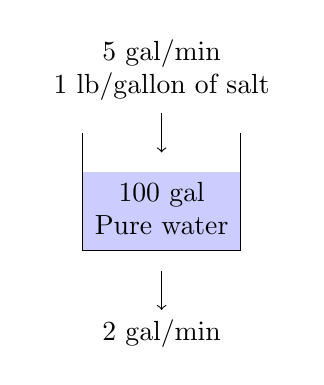
\begin{tikzpicture}[baseline = (current bounding box.north)]
		\draw[->] (1, -0.25) -- (1, -0.75) node[pos = 0, above] {\begin{tabular}{c} 5 gal/min \\ 1 lb/gallon of salt \end{tabular}};
		\fill[fill=blue!20!white] (0, -1) rectangle (2, -2);
		\draw (0, -0.5) -- (0, -2) -- (2, -2) -- (2, -0.5);
		\node at (1, -1.5) {\begin{tabular}{c} 100~gal \\ Pure water \end{tabular}};
		\draw[->] (1, -2.25) -- (1, -2.75) node[pos = 1, below] {2 gal/min};
	\end{tikzpicture}
\end{minipage}%
\begin{minipage}[t]{0.75\textwidth}
	\begin{center}
		(We assume the liquid in the tank is homogeneous at all times.)
	\end{center}
	We want to model the amount of salt in the container at any time. Let $x\p{t}$ be the number of pounds of salt at time $t$. While we can't model $x\p{t}$ directly, we can easily model its rate of change. To do so, we have to look at how much salt flows in and out over time. The rate of salt flow is simply the rate at which the solution flows in or out multiplied by the concentration of salt. In other words, it's the amount of salt that comes with the solution per unit time. Thus, we can model the rate of change of $x\p{t}$ as follows:
\end{minipage}
\begin{align*}
		\frac{\diff{x}}{\diff{t}} &= \text{(inflow of salt)} - \text{(outflow of salt)} \\
		&= \p{5~\frac{\text{gal}}{\text{min}} \cdot 1~\frac{\text{lb}}{\text{gal}}} - \p{2~\frac{\text{gal}}{\text{min}} \cdot \frac{x}{100 + \p{5 - 3}t}~\frac{\text{lb}}{\text{gal}}} \\
		&= 5~\frac{\text{lb}}{\text{min}} - \frac{2x}{100 + 2t}~\frac{\text{lb}}{\text{min}} \\
		&= 5 - \frac{x}{50 + t}
\end{align*}
Notice that the outflow of salt is a function of $x$ and $t$, which is because the amount of salt isn't constant and the amount of solution in the tank changes over time (at a constant rate in this problem).
\par\bigskip
The differential equation is linear with the initial condition $x\p{0} = 0$, meaning we can solve it using any of the techniques discussed in this chapter. We will use variation of parameters (Section 3.3.2).
\begin{align*}
	\frac{\diff{x_h}}{\diff{t}} &= -\frac{x_h}{50 + t} \\
	\int\frac{\diff{x_h}}{x_h} &= -\int\frac{\diff{t}}{50 + t} \\
	\ln{\abs{x_h}} &= -\ln{\abs{50 + t}} \\
	x_h &= \frac{1}{50 + t} \qquad \text{(both quantities are positive)}
\end{align*}
Our solution will be in the form $x = vx_h$, so substituting into the differential equation yields
\begin{align*}
	v'x_h + vx_h' &= 5 - \frac{vx_h}{50 + t} \\
	\frac{v'}{50 + t} - \cancel{\frac{v}{\p{50 + t}^2}} &= 5 - \cancel{\frac{v}{\p{50 + t}^2}} \\
	\frac{\diff{v}}{\diff{t}} &= 5\p{50 + t} \\
	v &= 250t + \frac{5}{2}t^2 + C
\end{align*}
Thus, the general solution to the mixing problem is given by \[ x\p{t} = \frac{250t + \frac{5}{2}t^{2} + C}{50 + t}. \] With the initial condition $x\p{0} = 0$, we get \[ \frac{C}{50} = 0 \implies C = 0, \] so the solution to the mixing problem is \[ x\p{t} = \frac{250t + \frac{5}{2}t^2}{50 + t} = \frac{500t + t^2}{100 + 2t}. \] A common variation to this problem is the addition to one or more tanks. In those problems, the outflow of one tank may be the inflow of another, but the overall setup will be the same. The main difference is that there will be more differential equations to solve, but they will all be linear.
	
\section{Exact Differential Equations}
\subsection{Introduction}
In this section, we will be dealing with differential equations of the form $P\p{x, y} + Q\p{x, y}y' = 0$, which we will write as $P\p{x, y}\,\diff{x} + Q\p{x, y}\,\diff{y} = 0$.

Our goal is to find a real-valued function $F\p{x, y}$ such that $F\p{x, y} = C$ implicitly defines a solution to the differential equation. To illustrate this, consider the following example.

\textit{Example:} \\
Let $P\p{x, y} = x$, $Q\p{x, y} = y$. We claim that the equation
\begin{equation}
	F\p{x, y} = x^2 + y^2 = C	
\end{equation}
implicitly defines a solution to the exact differential equation
\[
	x\,\diff{x} + y\,\diff{y} = 0.
\]
Taking the derivative with respect to $x$ on both sides of (1) yields
\begin{align*}
	2x + 2y\frac{\diff{y}}{\diff{x}} &= 0 \\
	2x\,\diff{x} + 2y\,\diff{y} &= 0 \\
	x\,\diff{x} + y\,\diff{y} &= 0
\end{align*}
as we wanted to show.

So, $x^2 + y^2 = C$ are solutions to the problem, which are circles of radius $\sqrt{C}$ centered at the origin.

\begin{definition}
	Suppose that the solutions for the differential equation $P\p{x, y} + Q\p{x, y}y' = 0$ are implicitly given by $F\p{x, y} = C$. Then the set $\left\{\p{x, y} \in \mathbb{R}^2 \mid F\p{x, y} = C \right\}$ are called the \textbf{integral curves} of the differential equation.	
\end{definition}



\end{document}
